% Chapter Template

\chapter{FDTD - One-Dimensional Scenario} % Main chapter title

\label{Chapter2} % Change X to a consecutive number; for referencing this chapter elsewhere, use \ref{ChapterX}

In this chapter, we will go more in depth into developing an application that can generate electromagnetic data in a one-dimensional domain. In the previous chapter, we mentioned a series of steps to implement FDTD, and that a part of them depend on the particular implementation. A keen eye will notice moving forward, that while the code will not change too much, each implementation deserves a different approach.

%----------------------------------------------------------------------------------------
%	SECTION 1
%----------------------------------------------------------------------------------------

\section{1D Discretization}



%-----------------------------------
%	SUBSECTION 1
%-----------------------------------
\subsection{Subsection 1}



%-----------------------------------
%	SUBSECTION 2
%-----------------------------------

\subsection{Subsection 2}


%----------------------------------------------------------------------------------------
%	SECTION 2
%----------------------------------------------------------------------------------------

\section{C++ Implementation}

\begin{minted}[breaklines,frame=single]{c++}
#define _USE_MATH_DEFINES

#include <iostream>
#include <stdio.h>
#include <math.h>
#include <stdlib.h>
#include <cmath>
#include <vector>
#include <string>

using namespace std;

const double permitivity = 8.854e-12;
const double permeability = 1.256e-6;

double L = 5;
int N = 200;
int iterNum = 800;
//double deltaX = L / N;
//double deltaY = L / N;
double deltaZ = L / N;
double deltaT = (deltaZ * sqrt(permitivity*permeability));

// variables needed for Gaussian Pulse excitation
double eps = 1e-3;
double Teps = 50 * deltaT;
double beta = -(pow((2/Teps), 2) * log(eps));


vector<double> E;
vector<double> H;
vector<double> tE;
vector<double> tH;

int main()
{
	E.assign(N, 0);
	H.assign(N, 0);
	
	
	for(int i = 0; i < iterNum; i++) {
		
		double t = i * deltaT;
		double gamma = Teps / 2;
		
		E[0] = exp(-(beta * pow((t - gamma), 2)));  //TO-DO: Gaussian excitation, alpha = 1, Teps = 50*deltaT, eps = 1e-3, t = i * deltaT
		
		// loop for values
		for (int z = 0; z < N-1; z++) {
			H[z] = H[z] - (deltaT / permeability / deltaZ) * (E[z] - E[z+1]);
		}
		
		for (int z = 1; z < N-1; z++) {
			E[z] = E[z] + (deltaT / permitivity / deltaZ) * (H[z] - H[z-1]);
		}
		
		
		// time graph
		tE.push_back(E[100]);
		tH.push_back(H[100]);
	}
	
	
	cout << "\n\ntE\n";
	
	// print E values
	for (int n = 0; n < iterNum; n++) {
		cout << to_string(tE[n]) + ",";
	}
	
	cout << "\n\ntH\n";
	
	// print H values
	for (int n = 0; n < iterNum; n++) {
		cout << to_string(tH[n]) + ",";
	}
	
}
\end{minted}

\section{Data Visualization}

\begin{figure}
	\centering
	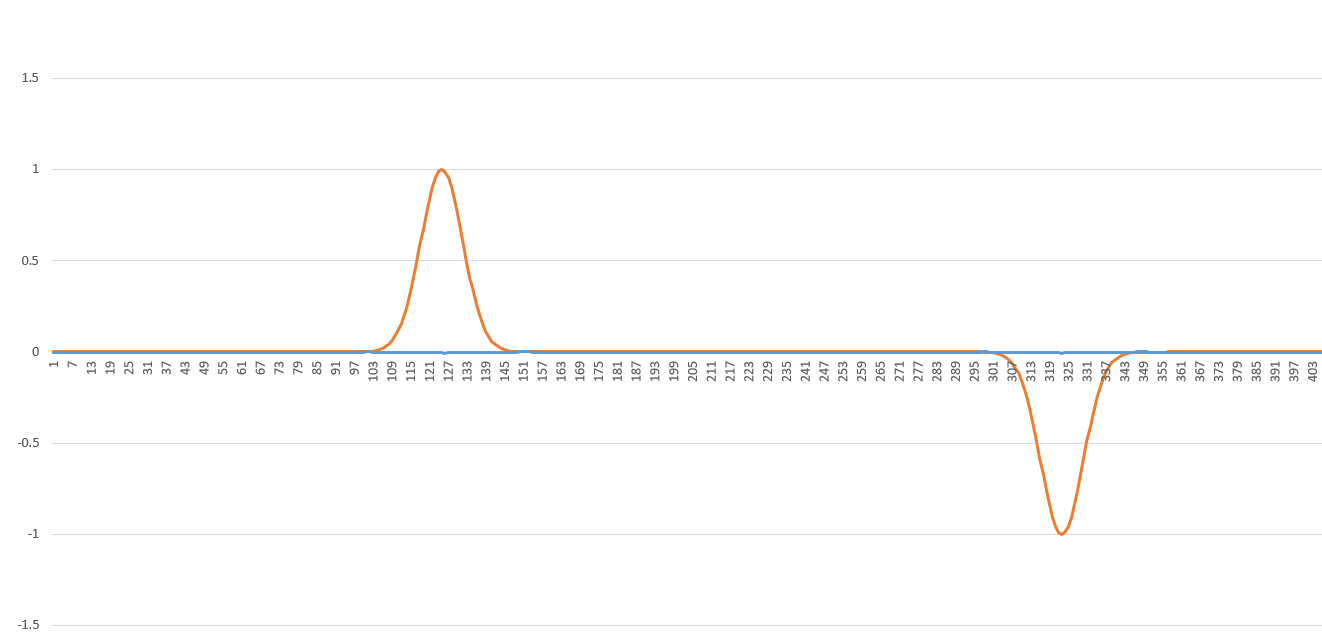
\includegraphics[scale=0.75]{Figures/1DtimeGraph1}
	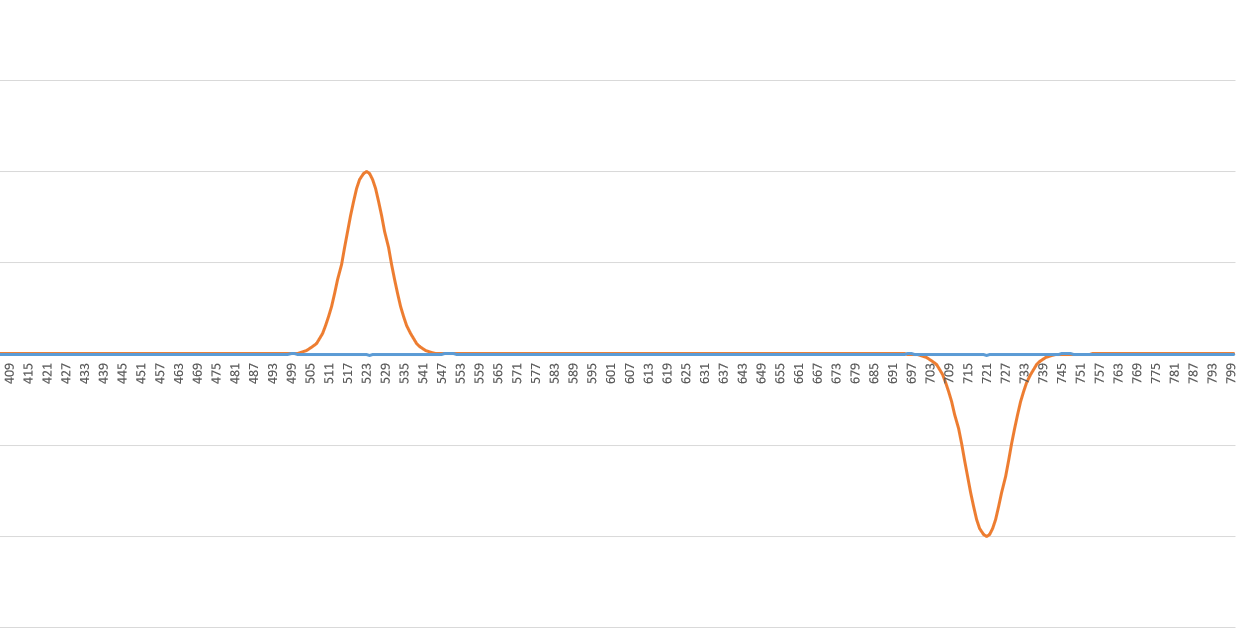
\includegraphics[scale=0.8]{Figures/1DtimeGraph2}
	\decoRule
	\caption[1D Electromagnetic Time Graph]{The time graph of the electromagnetic data generated by our 1D application.}
	\label{fig:emTimeGraph}
\end{figure}

\begin{figure}
	\centering
	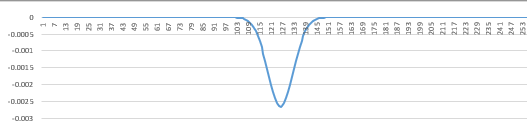
\includegraphics{Figures/1DmagneticTimeSnippet}
	\decoRule
	\caption[1D Magnetic Time Snippet]{A snippet of the time graph shown in Figure \ref{fig:emTimeGraph} zoomed in}
	\label{fig:mTimeSnippet}
\end{figure}